% chercher des documents LaTeX dans styles, corps et bib
\makeatletter\def\input@path{{styles/}{corps/}{bib/}}\makeatother

% Utiliser le style rapport.cls
\documentclass[12pt, a4paper]{report}

\usepackage[a4paper,vdivide={*,23cm,4cm}]{geometry}
\usepackage[russian, french]{babel} % style francais
\usepackage[encapsulated]{CJK}
\usepackage{styles/pageGardeEnsta}
\usepackage[T2A, T1]{fontenc}
\usepackage[utf8]{inputenc} % pour taper les accents directement
\usepackage{lmodern}
\usepackage{amsmath}
\usepackage{amsfonts}
\usepackage{amssymb}

\usepackage{tabularx}

\usepackage{caption}
\usepackage{subcaption}

\usepackage{titlesec}
%\titleformat*{\section}{\fontfamily{lmss}\selectfont\Large\bfseries}
\renewcommand{\thesection}{\Roman{section}.}
\titlespacing*{\section}{0pt}{\baselineskip}{.5\baselineskip}

\titleformat*{\subsection}{\fontfamily{lmss}\selectfont\large\bfseries}
\titlespacing*{\subsection}{1em}{.7\baselineskip}{.5\baselineskip}
\renewcommand{\thesubsection}{\arabic{section}.\arabic{subsection}.}
\renewcommand{\thesubsubsection}{\thesubsection\arabic{subsubsection}}
\titlespacing*{\subsubsection}{0pt}{.5\baselineskip}{.3\baselineskip}

\renewcommand{\labelenumi}{\textbf{\arabic{enumi}.}}

\renewcommand{\phi}{\varphi}


%\usepackage{fourier}

\usepackage[hidelinks]{hyperref}

% chemistry
\usepackage[version=3]{mhchem}

\graphicspath{{imgs/}}
% liens hypertexte dans le document
\usepackage{xcolor}
\usepackage{textcomp}

\usepackage{lastpage}

\usepackage{pgf-umlcd}

\usepackage{fancyhdr}
\pagestyle{fancy}
\fancyhf{}
\fancyhead[L]{}
\fancyhead[C]{}
\fancyhead[R]{Projet découverte de système}
\fancyfoot[L]{}
\fancyfoot[C]{}
\fancyfoot[R]{Page \thepage{} sur~\pageref{LastPage}}

\usepackage{lscape}
\usepackage{booktabs}


\title{Positionnement GNSS : du mètre au millimètre}
\author{}
\date{\today}
\doctype{Projet découverte de système}
\promo{FISE 2024}
\etablissement{\textsc{Ensta} Bretagne\\ 2, rue François Verny\\
   29806 \textsc{Brest} cedex\\ \textsc{France}}
\logoEcole{
\includegraphics[height=4.2cm]{logo_ENSTA_Bretagne_Vertical_CMJN}}


\newcommand{\ie}{\textit{i.e.}}

\begin{document}

\maketitle

   \section*{Introduction}
   Nous avons, dans le cadre du projet de découverte de système, du semestre 2 de notre scolarité à l'ENSTA Bretagne, mené une étude des systèmes GNSS (\textit{Global Navigation Satellite Systems}).

   Les objectifs sont premièrement une compréhension des systèmes de positionnement par satellite et de leur transmission de données par une étude bibliographique préalable, puis la conduite d'une campagne de mesures à partir de deux récepteurs différents.
   Le tout ayant comme finalité de visualiser les données acquises, mais aussi et surtout de conclure sur une étude métrologique comparative des deux récepteurs afin d'en obtenir différences en termes de précision du positionnement.

   \vspace{3cm}
   \begin{center}
   * \\
   *  \ \ *\\
   \end{center}

   \tableofcontents

   \section{Mise en contexte bibliographique}\label{sec:mise-en-contexte-bibliographique}
   \subsection{GNSS : les origines}\label{subsec:gnss-les-origines}
      Les GNSS (\textit{Global Navigation Satellite Systems}) sont des constellations de satellites conçues afin de fournir un positionnement et un chronométrage d'informations à destination des utilisateurs aussi bien sur Terre que dans l'espace.
      Ils sont utilisés pour générer une estimation de la position, de la vitesse et du temps en traitant les signaux transmis par des satellites d'orbites connues.

      Il existe de nos jours quatre types de systèmes GNSS : GPS, GLONASS, GALILEO et BEIDOU~\cite{gebre-egziabherGNSSApplicationsMethods2009}.

      \subsubsection{Le GPS}
         Actuellement, la constellation la plus utilisée à l'échelle mondiale est le GPS (\textit{Global Positioning System}), conçu par le département de la défense des États-Unis à des fins militaires.
         Le déploiement du système GPS a débuté le 22 février 1978 avec le lancement du premier satellite \textit{Bloc I Navstar GPS}.
         Sa capacité opérationnelle initiale a été annoncée en décembre 1993, pas moins de 24 satellites GPS répartis sur 6 orbites.

      \subsubsection{Le GLONASS}
         En supplément du GPS, un autre système pleinement opérationnel est le GLONASS (\textit{\foreignlanguage{russian}{глобальная навигационная спутниковая система}, Globalnaïa Navigatsionnaïa Spoutnikovaïa Sistéma}) de la Fédération de Russie.
         Ce programme, né dans les années 1980, est devenu opérationnel en 1995 avec une constellation également composée de 24 satellites sur 6 orbites.

         Cependant, la chute de l'URSS a entraîné une baisse drastique des fonds alloués au système GLONASS ayant pour conséquence sa dégradation.
         Depuis 2001, on compte au nombre de 6 les satellites encore opérationnels.

      \subsubsection{Galileo}
         L'Europe, cherchant à affirmer sa souveraineté, tente de s'affranchir des systèmes GPS et GLONASS au travers du projet Galileo, imaginé entre 1999 et 2000 par 4 membres de l'Union Européenne (France, Allemagne, Italie et Royaume-Uni).

         Le système Galileo devrait être opérationnel à l'horizon 2024, fort d'une constellation de 30 satellites répartis sur 3 orbites.

      \subsubsection{Beidou}
         La Chine a également mis en place, à partir de 2000, son propre GNSS appelé Beidou (\textit{\begin{CJK}{UTF8}{gbsn}北斗\end{CJK}}).
         Cette constellation est pleinement opérationnelle depuis le 23 juin 2020, totalisant 35 satellites sur 3 orbites.

   \subsection{Applications}\label{subsec:applications}
      Des applications pratiques des GNSS se retrouvent dans un large spectre de domaines, aussi bien pour des problématiques de positionnement que de synchronicité temporelle.

      On présente alors une liste non exhaustive de domaines et d'exemples d'applications des GNSS\@ :

      \vspace{1em}

      \begin{tabularx}{.95\textwidth}{|l|X|}
         \hline
         \textbf{Domaines d'utilisation} & \textbf{Exemples de missions} \\
         \hline
         Gestion de ressources & Sauvegarde de la faune et la flore, surveillance des ressources en eau\dots \\
         \hline
         Marin & Navigation marine, entretien des voies navigables \\
         \hline
         Topographie et géologie & Mesure de la déformation des volcans, des mouvements des plaques tectoniques\dots \\
         \hline
         Navigation & Guidage automobile, agriculture de précision, pêche de précision, guidage aéronautique, lutte contre le vol\dots \\
         \hline
         Militaire & Positionnement de l'ennemi et des toupes alliées, simulation de portée (missiles), guidage \\
         \hline
         Génie civil & Cartographie, systèmes d'arpentage \\
         \hline
         Horlogerie & Synchronisation sur le temps universel \\
         \hline
      \end{tabularx}

   \subsection{Méthode de positionnement}\label{subsec:methode-de-positionnement}
      Le positionnement consiste en la détermination de la position exacte d'un récepteur par un ou plusieurs systèmes GNSS\@.
      Pour y parvenir, trois inconnues sont à déterminer : la latitude, la longitude et l'altitude.

      En réalité, le calcul de ces coordonnées étant permis par des mesures de temps de trajet d'ondes électromagnétiques, il est nécessaire pour les satellites et le récepteur de synchroniser leurs horloges.
      Ainsi, un minimum de 4 satellites seront nécessaires afin de déterminer une position : 3 satellites pour le positionnement spatial, et un quatrième permettant la synchronisation des horloges~\cite{bosserGNSSSystemesGlobaux2017}.

      \subsubsection{Détermination de la distance entre satellite et récepteur}
         Les systèmes GNSS se composent de plusieurs dizaines de satellites évoluant à environ vingt-mille kilomètres d'altitude suivant des orbites impartialement réparties pour couvrir tous les continents.
         Cette couverture permet à un récepteur GNSS (téléphone, automobile, aéronautique\dots) de percevoir en moyenne entre cinq et trente-cinq satellites (GPS, GLONASS ou Beidou) en fonction de sa position.
         Chaque satellite enverra alors en continu sa position, et le temps d'émission de cette position (déterminée avec une horloge atomique embarquée sur le satellite).

         Ces informations, permettront alors, en connaissant les temps de réception et d'émission et la vitesse de propagation de l'onde électromagnétique émise par le satellite, de calculer la distance séparant le récepteur à celui-ci.

      \subsubsection{Détermination de la latitude et de la longitude}
         Grâce à la distance mesurée entre le récepteur et un certain nombre de satellites, il est posible de déterminer avec précision la position du récepteur.

         En effet, le récepteur mesurant une distance $d$ le séparant d'un satellite se situe quelque part sur une boule de rayon $d$ autour de ce satellite.

         \begin{figure}[h]
             \centering
             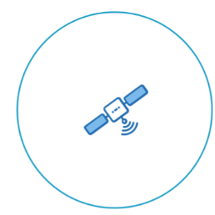
\includegraphics[width=.3\textwidth]{imgs/sat1}
             \caption{Un premier satellite}
             \label{fig:1sat}
         \end{figure}

         En se munissant d'un second satellite, de distance connue, on peut de la même manière tracer autour de sa position une boule de rayon égal à cette distance.

         \begin{figure}[h]
             \centering
             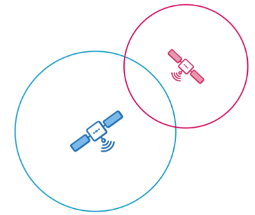
\includegraphics[width=.3\textwidth]{imgs/sat2}
             \caption{Deux satellites}
             \label{fig:2sat}
         \end{figure}

         Et finalement, la même opération sur un troisième satellite permettra au récepteur d'identifier l'unique point d'intersection entre les boules, correspondant à sa position.

         \begin{figure}[h]
             \centering
             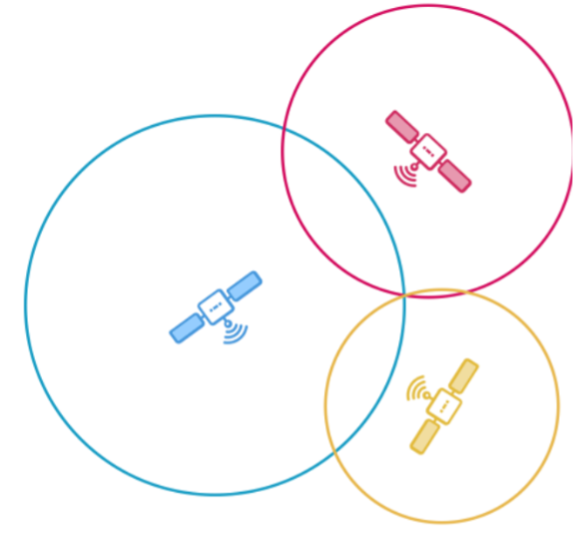
\includegraphics[width=.3\textwidth]{imgs/sat3}
             \caption{3 satellites, détermination de position}
             \label{fig:3sat}
         \end{figure}

         Il est alors très logiquement possible d'affiner ce résultat en augmentant le nombre de satellites, ou encore la précision de la mesure du temps du récepteur par exemple.

         \begin{figure}[h]
             \centering
             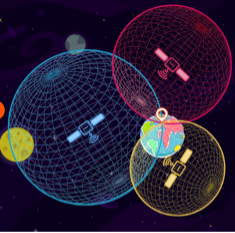
\includegraphics[width=.5\textwidth]{imgs/sat-3D}
             \caption{Représentation en 3D}
             \label{fig:repr3d}
         \end{figure}

      \subsubsection{Synchronicité des horloges}
         La détermination de la distance entre le récepteur et les satellites étant intrinsèquement liée à un repère d'horloge, une synchronisation temporelle entre les satellites et le récepteur est nécessaire (une erreur de l'ordre du millionième de seconde entraîne une erreur de positionnement de l'ordre de la centaine de mètres !).

         Pour résoudre ce problème, un quatrième satellite est nécessaire, permettant de se munir d'une donnée temporelle précise (grâce à son horloge atomique embarquée), permettant alors au récepteur de compenser les différences d'horloge afin d'affiner son positionnement jusqu'à en obtenir une valeur précise et juste~\cite{gebre-egziabherGNSSApplicationsMethods2009}.

      \subsubsection{Facteurs influençant le positionnement par satellite}
         Il est cependant à noter que divers facteurs tels que le niveau d'humidité, les variations de pression ou encore le rayonnement solaire peuvent modifier la vitesse ou la direction des signaux émis par les satellites, introduisant des erreurs dans les mesures.

         On comprend donc l'utilité de se munir d'un grand nombre de satellites afin de s'assurer d'une bonne précision.

   \subsection{Lecture de données GNSS}\label{subsec:lecture-de-donnees-gnss-format-nmea}
      \subsubsection{Format NMEA}
         Le format NMEA (\textit{National Marine Electronics Association}) a été proposé en 1983 par la marine nationale américaine afin de permettre la standardisation des communications entre les équipements marins, dont les émetteurs / récepteurs GPS\@.
         Ce format permet d'échanger facilement diverses informations de positionnement et de calibrage entre plusieurs appareils, faisant \textit{de facto} du format NMEA une norme pour les différents GNSS~\cite{hofmann-wellenhofGNSSGlobalNavigation2007}.

      \subsubsection{Lecture d'une trame NMEA}
         Une trame NMEA débute nécessairement par un symbole \texttt{\$} directement suivi du système GNSS reçu (GP pour le GPS, GL pour le GLONASS\dots) et l'intitulé de la donnée (code de 5 lettres).
         Suivent alors, séparées par des virgules, les données reçues.

         On donne l'exemple d'une trame GGA reçue par le système GPS, et on remarquera en particulier le \textit{checksum}, clé de contrôle permettant de vérifier la validité des données :

         \begin{figure}[h]
             \centering
             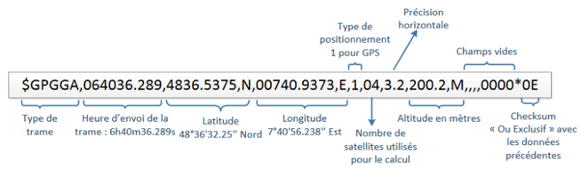
\includegraphics[width=.95\textwidth]{imgs/trame-gga}
             \caption{Exemple de trame GGA}
             \label{fig:trame-gga}
         \end{figure}


   \section{Récepteurs étudiés et acquisition}\label{sec:recepteurs-etudies-et-acquisition}
   Notre étude est orientée autour de deux récepteurs GNSS de coût et capacités différentes, l'un étant supposé être plus précis que l'autre.
   Nous allons donc chercher à prendre des mesures à l'aide de ces deux récepteurs afin de les étudier et entre autres de vérifier cette supposition.

   \subsection{Premier récepteur}\label{subsec:premier-recepteur-:-gpstar}
      Le premier récepteur, qui est celui que nous avons le plus utilisé lors de la prise de mesures, est le G Star IV de la marque \textit{GlobalSat}.
      Il s'agit d'un récepteur uniquement GPS, de petite taille, ce qui en fait un outil portable relativement précis permettant aisément d'effectuer des relevés de position grâce à un ordinateur.

      \begin{figure}[h]
          \centering
          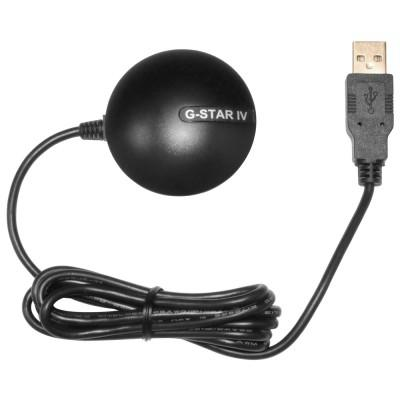
\includegraphics[width=.4\textwidth]{imgs/gstar}
          \caption{Récepteur G Star IV}
          \label{fig:gstar}
      \end{figure}

      Une fois branché en USB à un ordinateur, il est possible d'exploiter ses prises de mesures.
      Le récepteur transmettant les données reçues depuis les satellites émetteurs sous forme de suite de bits qu'il est possible de lire grâce au module \texttt{Serial} de Python, il est cependant nécessaire d'effectuer une traduction afin de rendre les données exploitables.

      En effet, les données sont donc transmises \textit{via} USB comme une suite de bits.
      Il faut donc tout d'abord organiser ces bits en octets, puis convertir chaque octet en valeur associée à un caractère de texte encodé selon la norme UTF-8.

      Une fois les données converties, il est intéressant de remarquer qu'elles suivent le format NMEA\@.
      Nous les enregistrons donc dans un fichier texte qu'il sera possible d'exploiter ultérieurement.

   \subsection{Second récepteur}\label{subsec:second-recepteur}
      Le second récepteur étudié est le SP80 de \textit{Spectra Geospatial}.
      Contrairement au premier récepteur, il est bien plus précis mais surtout bien plus imposant.
      Il possède, de plus, la capacité de recevoir des données aussi bien depuis le système GPS que depuis les systèmes GLONASS et Beidou.

      \begin{figure}[h]
          \centering
          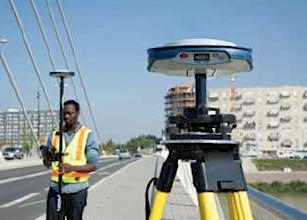
\includegraphics[width=.45\textwidth]{imgs/sp80}
          \caption{Récepteur SP80}
          \label{fig:sp80}
      \end{figure}

      Il se place alors naturellement comme un récepteur GNSS à usage d'avantage professionnel, pour des opérations nécessitant une précision conséquente.

      Concernant l'acquisition, le procédé est similaire, la transmission par USB s'effectuant de la même manière.

   \section{Lecture des acquisitions et premiers résultats}\label{sec:lecture-des-acquisitions-et-premiers-resultats}
   Maintenant que nous savons utiliser les récepteurs GNSS et enregistrer les mesures ainsi prises dans un fichier au format NMEA, vient désormais le moment de lire ces données avec Python afin de pouvoir les exploiter.

   \subsection{Implémentation}\label{subsec:implementation}
      Afin de rendre l'exploitation des données plus simple, plusieurs choix techniques ont été pris.
      Tout d'abord, la programmation en Python qui nous a paru adaptée à la forme du problème, le langage permettant facilement de traiter des données numériques contenues dans un fichier texte.

      Deuxièmement, il a été décidé de concevoir un programme orienté-objet, et donc d'implémenter une classe \texttt{Data} dans laquelle seront stockées les données contenues dans un fichier NMEA, ce qui permet alors, à partir d'une unique lecture des données du fichier d'acquisition, d'opérer différentes exploitations.
      Ainsi, il est possible à partir d'un simple fichier contenant des données NMEA d'instancier un objet \texttt{Data} qui en extraira l'ensemble des données à son initialisation.
      Il est alors possible d'opérer diverses opérations telles que le tracé d'un chemin GPS ou encore une étude métrologique comparative entre deux objets \texttt{Data} distincts, le tout en lisant une seule fois les données depuis le fichier texte.

      Nous allons donc, par la suite, détailler quelques opérations effectuées sur les données acquises.


   \subsection{Nettoyage des données}\label{subsec:nettoyage-des-donnees}
      Une première opération pouvant être effectuée sur les données est un \og nettoyage \fg{} de ces dernières, permettant de transformer les données brutes en des données pouvant être extraites vers une liste Python, permettant également le transtypage de données numériques en entiers ou flottants.

   \subsection{Visualisation des données}\label{subsec:visualisation-des-donnees}
      Une première visualisation des données possible à partir des données NMEA est, à partir des trames GGA (position du récepteur), l'évolution de la position du récepteur GNSS en deux dimensions (latitude et longitude).
      Ainsi, très simplement, les coordonnées extraites des trames GGA sont converties du format sexagésimal au format décimal afin d'être placées dans un repère 2D par le module \texttt{matplotlib} de Python, mais il est aussi possible de prendre en compte l'altitude, renseignée dans les trames GGA, pour obtenir un tracé en 3 dimensions.

      \begin{figure}[h]
          \centering
          \begin{subfigure}[h]{.45\textwidth}
             \centering
             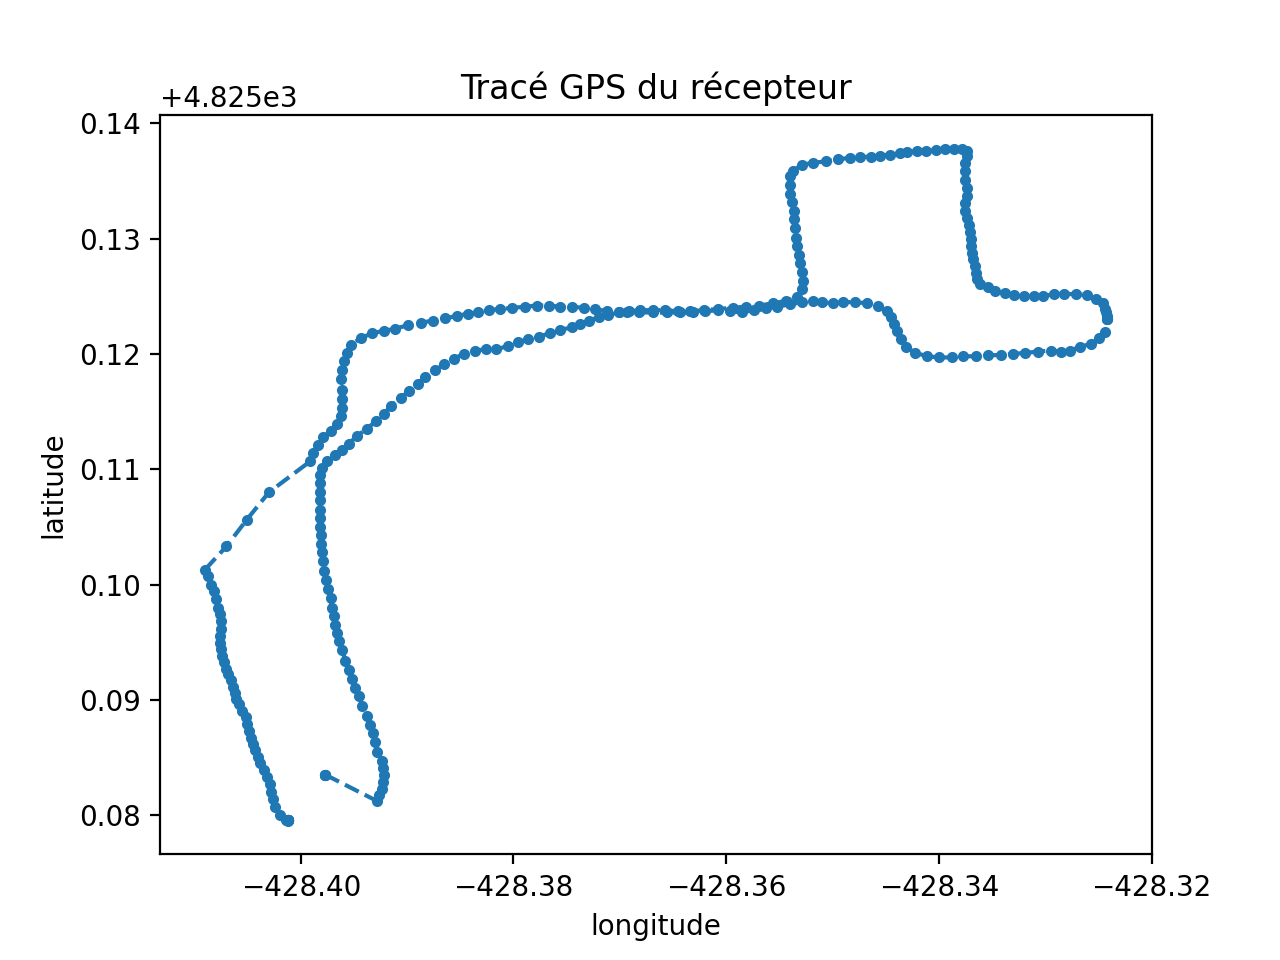
\includegraphics[width=\textwidth]{imgs/coords_2d}
          \end{subfigure}
          \hfill
          \begin{subfigure}[h]{.45\textwidth}
             \centering
             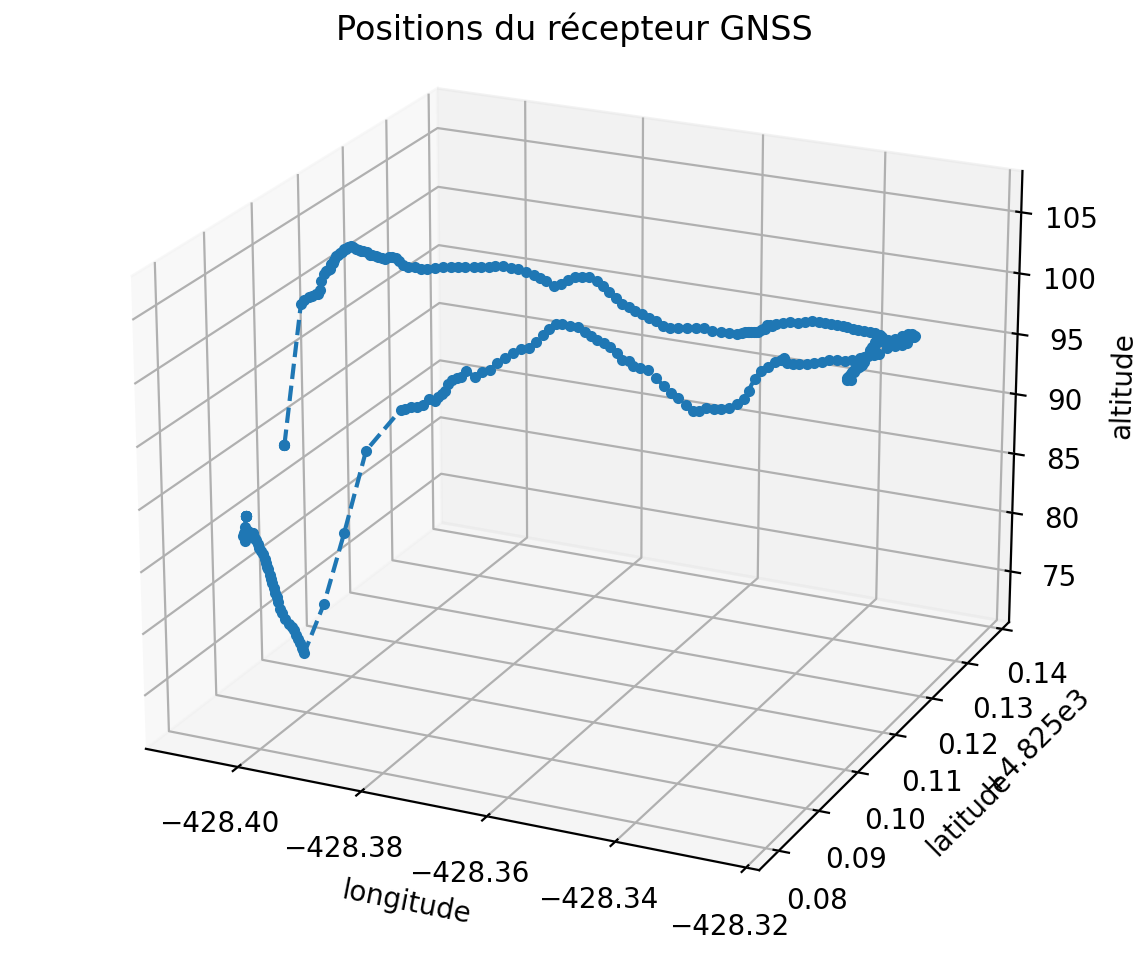
\includegraphics[width=\textwidth]{imgs/coords_3d}
          \end{subfigure}
          \caption{Position du récepteur en 2D et 3D}
          \label{fig:plot-coords}
      \end{figure}

      Mais il est également possible, grâce au module \texttt{folium}, d'obtenir la même représentation, mais sur un fond de carte\footnote{le fond de carte est celui d'\texttt{openstreetmap}} dans un fichier HTML (il est donc possible de naviguer sur la carte, sur laquelle est affiché le tracé des coordonnées successives du récepteur).

      \begin{figure}[h]
          \centering
          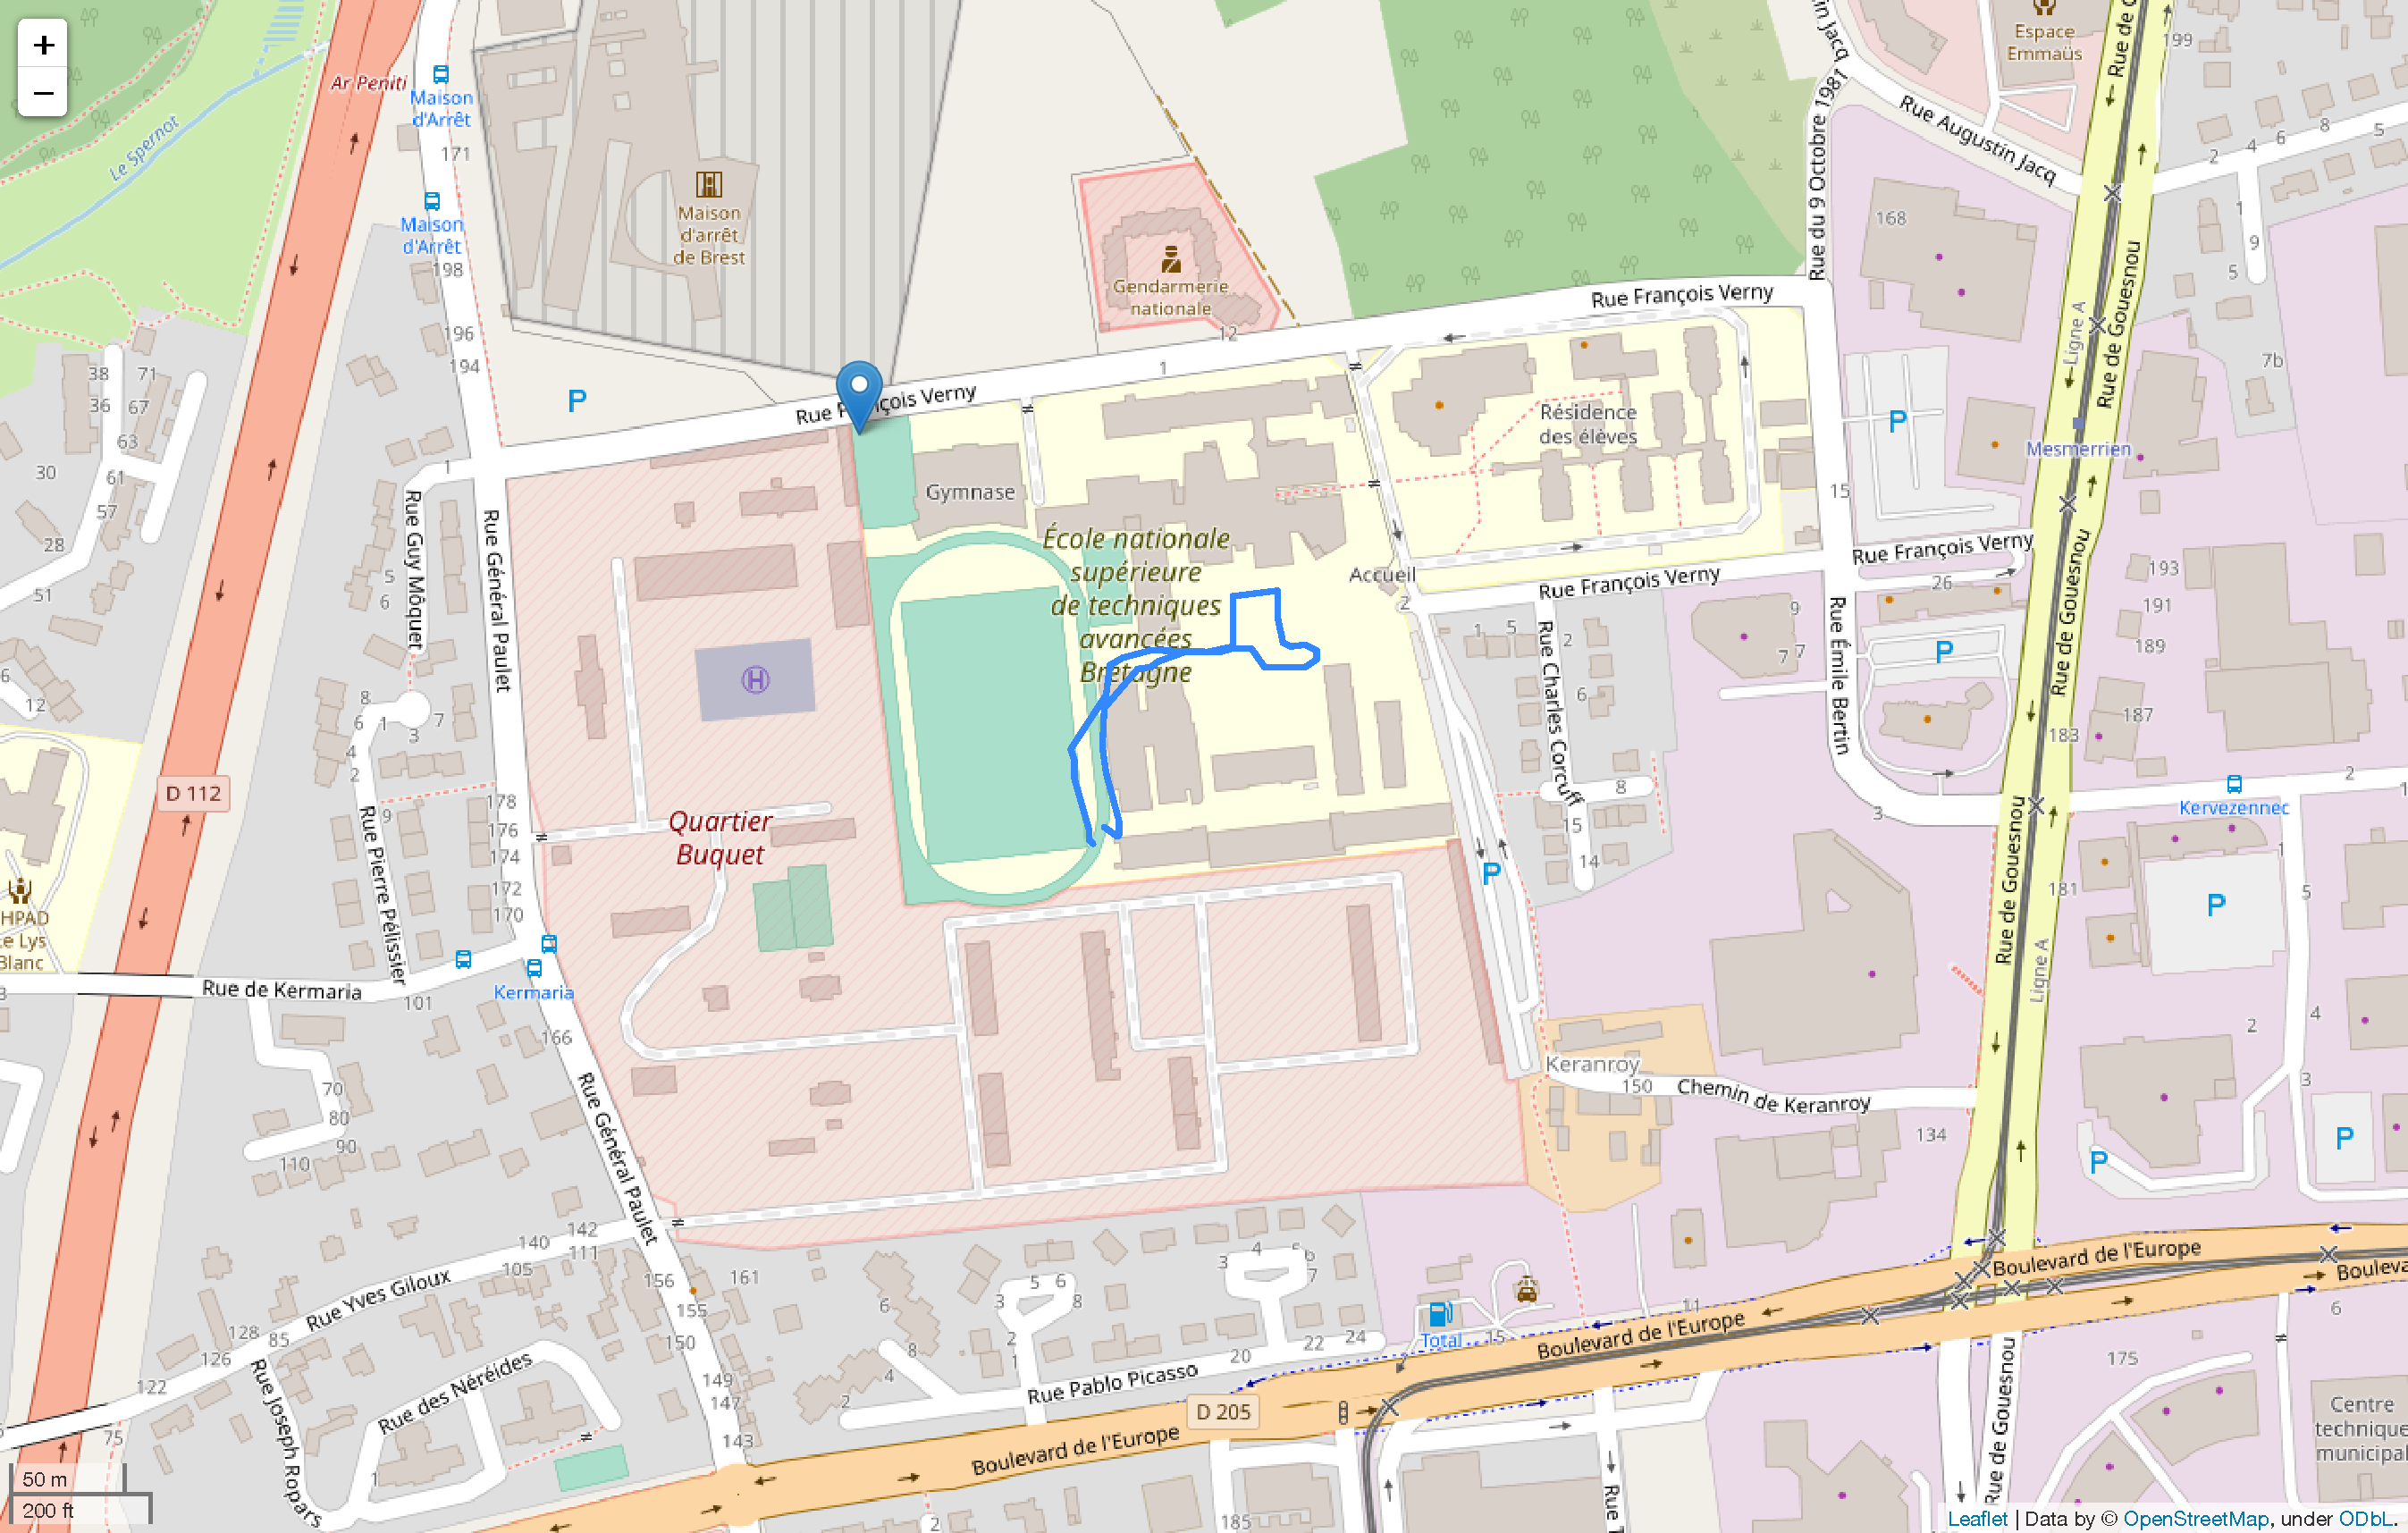
\includegraphics[width=.9\textwidth]{imgs/gps_map}
          \caption{Trace GPS sur un fond de carte HTML}
          \label{fig:coords-on-map}
      \end{figure}



   \section{Visualisation des satellites}\label{sec:visualisation-des-satellites}
   Afin d'affiner notre compréhension du système GNSS, et nous aider à mieux le visualiser, déterminer l'origine des mesures en exploitant les données sur les satellites émetteurs nous a semblé indispensable.
   En effet, les constellations de satellites utiles au positionnement assurent continument un service de géolocalisation autour du monde.
   Ainsi, à tout moment, des satellites émettent des données pouvant être lues par un récepteur.

   Pour nous donner une petite idée de cette disponibilité des satellites, tracer depuis un fichier NMEA la position des satellites ayant servi au positionnement (trames GSV) nous semble être une manière intéressante de procéder.
   Il est alors nécessaire de pouvoir remonter des données brutes enregistrées par le récepteur à la position des satellites autour de la Terre.

   \subsection{Récupération des données}\label{subsec:recuperation-des-donnees}
      La première étape est donc d'extraire du fichier NMEA les information sur les satellites émetteurs.
      Pour cela, nous allons extraire les trames GSV et en extraire les informations, à savoir le nombre de satellites disponibles, et pour chacun sa position en azimut et élévation ainsi que la force du signal.
      La méthode \texttt{satellite\_pos} permet donc cette extraction des données en les organisant dans une matrice de transmission contenant toutes ces caractéristiques sur les satellites.

      \begin{figure}[h]
          \centering
          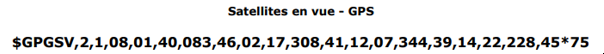
\includegraphics[width=.95\textwidth]{imgs/gsv}
          \caption{Exemple de trame GSV}
          \label{fig:gsv}
      \end{figure}

   \subsection{Tracé dans le référentiel de l'observateur}\label{subsec:trace-dans-le-referentiel-de-l'observateur}
      Une fois les données extraites, nous avons souhaité, dans un premier temps, positionner ces satellites dans une carte du ciel vue de la position du récepteur.

      Tout d'abord, les coordonnées horizontales sont converties en coordonnées sphériques locales centrées sur le récepteur GNSS\@.
      En effet, en orientant l'axe des abscisses vers l'Est, l'axe des ordonnées vers le Nord et les cotes vers les altitudes croissantes, on obtient une vue des satellites dans le ciel en faisant correspondre l'azimut avec l'angle $\pi/2 - \phi$ et l'élévation avec l'angle $\theta$.
      Le rayon $r$ sera déterminé arbitrairement.

       \begin{figure}[h]
             \centering
             \begin{subfigure}[h]{.45\textwidth}
                \centering
                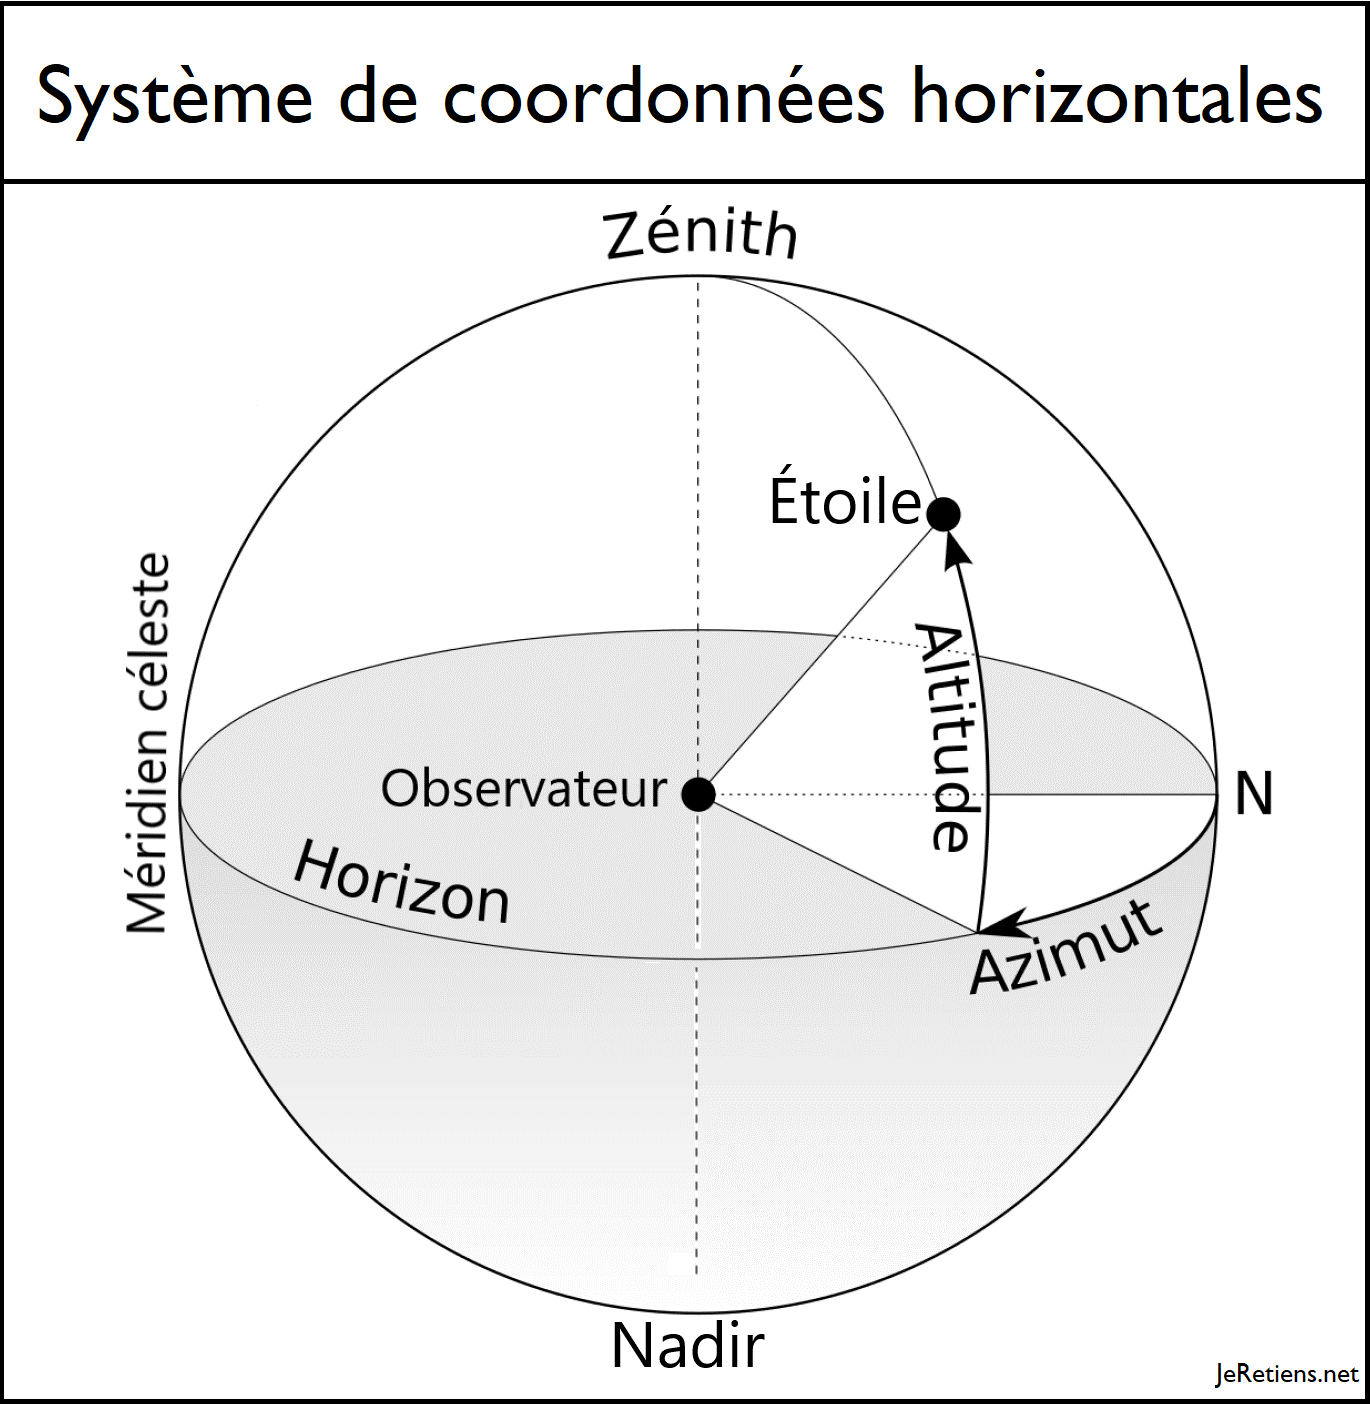
\includegraphics[width=\textwidth]{imgs/horizon}
             \end{subfigure}
             \hfill
             \begin{subfigure}[h]{.45\textwidth}
                \centering
                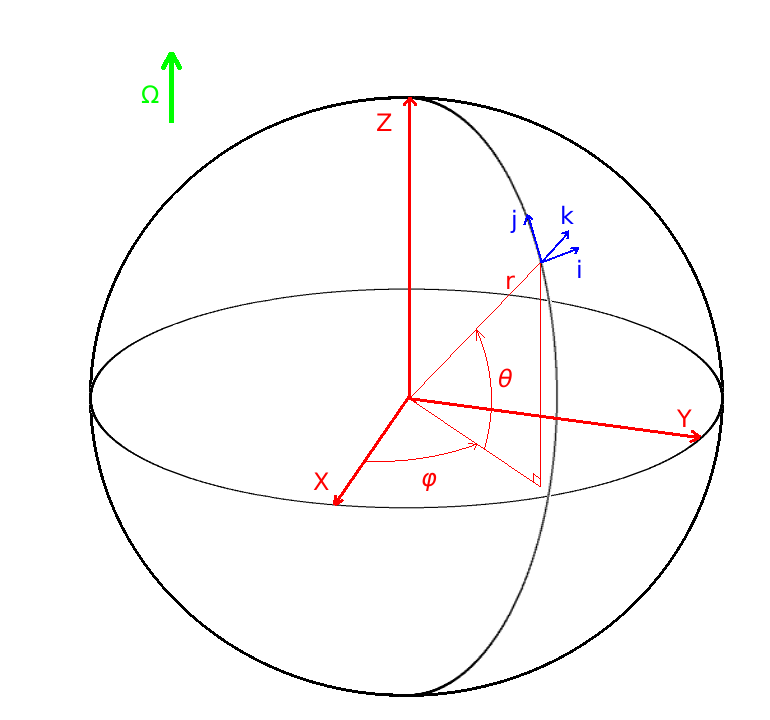
\includegraphics[width=\textwidth]{imgs/geo}
             \end{subfigure}
             \caption{Systèmes de coordonnées a) horizontales et b) géométriques}
             \label{fig:coords-terre}
         \end{figure}

      Puis, pour programmer le tracé dans Python, nous utilisons les coordonnées cartésiennes obtenues par :
      \[\begin{cases}
           x = r\sin\theta\cos\phi \\
           y = r\sin\theta\sin\phi \\
           z = r\cos\theta \\
      \end{cases}\]
      le tout réalisé par la méthode \texttt{plot\_satellite}.

      \begin{figure}[h]
          \centering
          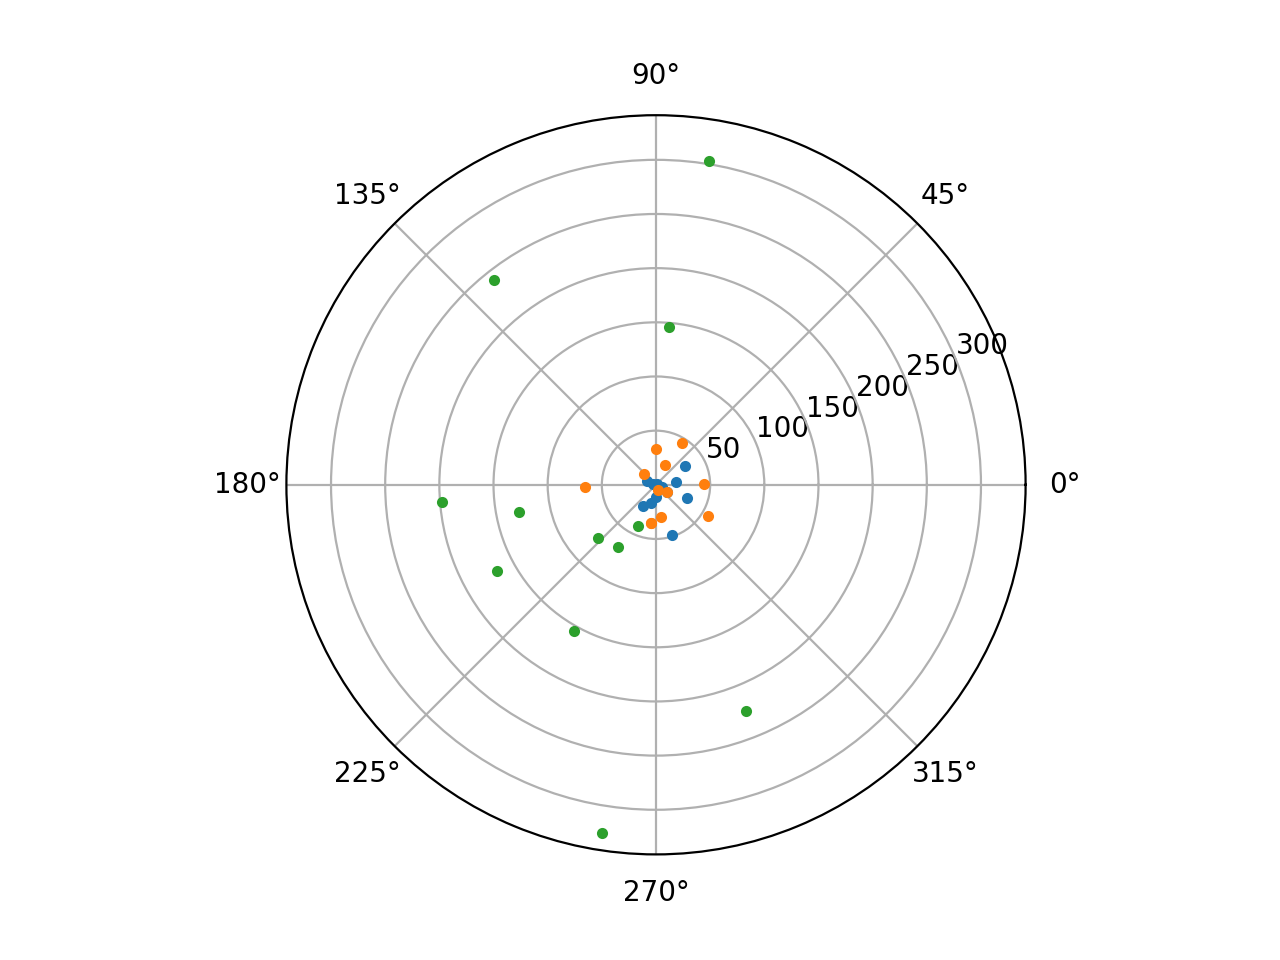
\includegraphics[width=.7\textwidth]{imgs/satpolar}
          \caption{Carte céleste des satellites}
          \label{fig:polarsat}
      \end{figure}

   \subsection{Tracé dans le référentiel géocentrique}\label{subsec:trace-dans-le-referentiel-geocentrique}
      Enfin, pour nous munir d'une représentation d'avantage complète et visuelle du positionnement des satellites en orbite, il nous a semblé judicieux de les placer dans le repère géocentrique.
      Il sera donc nécessaire de convertir les coordonnées horizontales obtenues précédemment.

      Nous devons donc effectuer la conversion du système de coordonnées ENU (\textit{East North Up}), qui est dans le plan local tangent à la Terre (correspondant au repère cartésien du système de coordonnées précédemment introduit) dans le système de coordonnées ECEF (\textit{Earth Centered Earth Fixed}) correspondant au repère cartésien géocentré.
      \begin{center}
         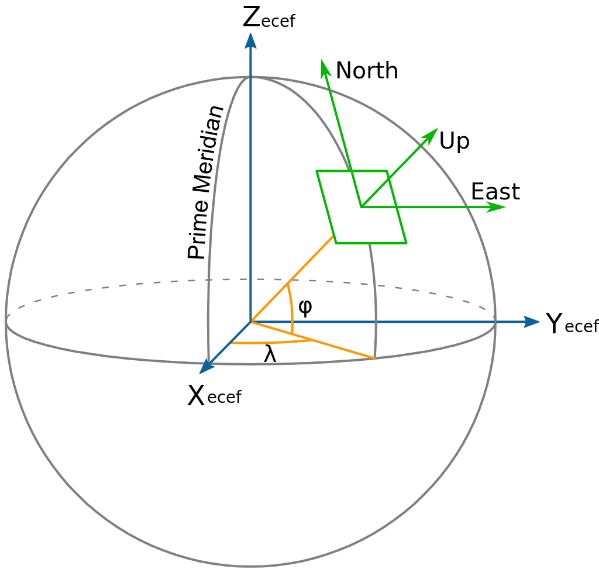
\includegraphics[width=.35\textwidth]{imgs/enutoecef}
      \end{center}

      La conversion est effectuée par le produit matriciel :
      \[
         \begin{pmatrix}
            X \\
            Y \\
            Z
         \end{pmatrix} =
         \begin{pmatrix}
            -\sin\lambda & -\sin\phi\cos\lambda & \cos\phi\cos\lambda \\
            \cos\lambda  & -\sin\phi\sin\lambda & \cos\phi\sin\lambda \\
            0            & \cos\phi             & \sin\phi
         \end{pmatrix}
         \begin{pmatrix}
            x \\
            y \\
            z
         \end{pmatrix}
      \]

      Grâce à la matrice de conversion, il est donc possible de déterminer les nouvelles coordonnées des satellites, puis de tracer en trois dimensions la position du récepteur sur la Terre, puis la position des satellites en orbite (d'altitude fixée arbitrairement pour la visualisation).

      \begin{figure}[h]
          \centering
          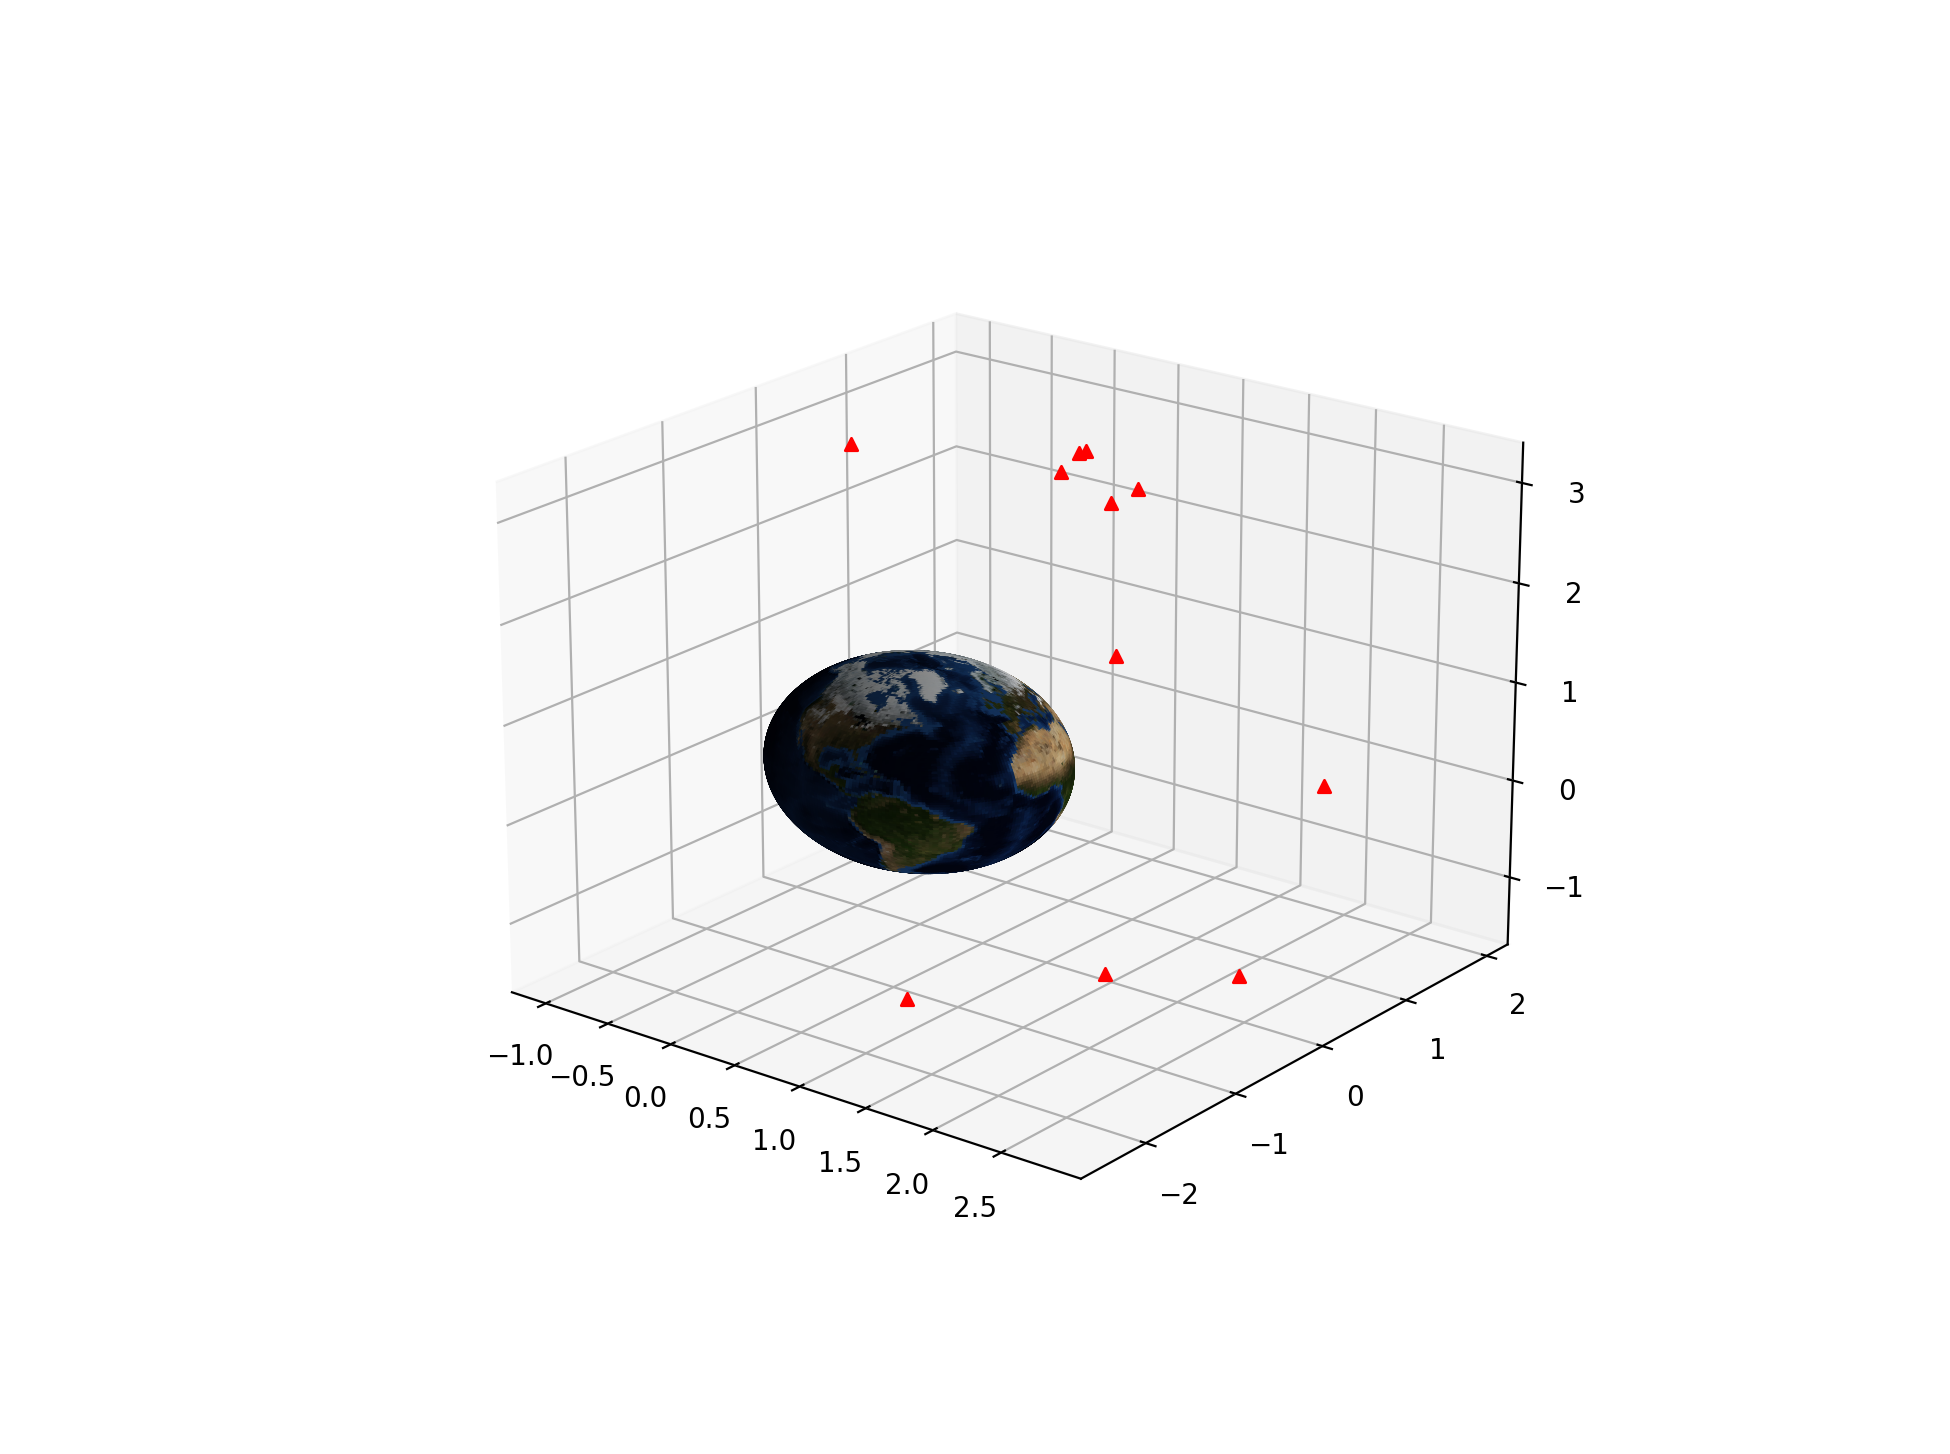
\includegraphics[width=.7\textwidth]{imgs/visuplanet}
          \caption{Résultat de la méthode \texttt{visu\_planet}}
          \label{fig:visuplanet}
      \end{figure}

   \include{corps/métrologie}

   \section*{Conclusion}
   Finalement, grâce à ce projet de découverte de système, nous avons pu comprendre de manière approfondie le fonctionnement d'un système aussi commun que complexe, à savoir le positionnement par satellite.

   Il nous a alors été possible de saisir les subtilités du positionnement géographique mais aussi des protocoles de transmission, permettant de passer d'un flot de données binaires à un fichier au format standardisé pouvant être traité et visualisé.

   À ce titre, ce projet a été l'occasion pour nous d'approfondir nos capacités de traitement de données et de visualisation en Python, tout en développant un goût pour les mesures géographiques.

   Finalement, l'étude métrologique aura apporté des résultats numériques à nos attentes théoriques, ce qui aura permis de caractériser les deux récepteurs étudiés, en créant une correspondance entre les mesures expérimentales et les principes théoriques.

   \vspace{3cm}
   \begin{center}
   *  \ \ *\\
   *
   \end{center}

   % Lorem ipsum
% %
%   \begin{landscape}
   \section*{Annexe II. Fonctionnement schématique d'une partie côté \textit{backend}}
   \addcontentsline{toc}{section}{Annexe II. Fonctionnement \textit{backend} d'une partie}
   \begin{center}
      \includegraphics[height=.92\textwidth]{imgs/actDiagram}
   \end{center}
\end{landscape}


   % \include{corps/back}

   \bibliographystyle{plain}
   % \bibliographystyle{ieeetr}
   \bibliography{bib/biblio}
   \addcontentsline{toc}{section}{Références}



   \listoffigures
   \addcontentsline{toc}{section}{Liste des figures}

   \section*{Annexe -- Résultats numériques}
\addcontentsline{toc}{section}{Annexe -- Résultats numériques}

   \begin{table}[h]
       \centering
       \begin{tabular}{l|ccc}
           \toprule
           \textbf{} & \textbf{Moyenne} & \textbf{Écart-type} & \textbf{Incertitude-type} \\
           \midrule
           Longitude & -4.47423527 & 8.69581991e-07 & 1.468878e-07 \\
           Latitude & 48.41905494 & 2.99175820e-07 & 5.056994e -08 \\
           \midrule
           Distance à référence & $2.387\, \mathrm{m}$ & & \\
           \bottomrule
       \end{tabular}
       \caption{Récepteur le moins précis}
       \label{tab:recept-pas-precis}
   \end{table}

    \begin{table}[h]
        \centering
        \begin{tabular}{l|ccc}
            \toprule
            \textbf{} & \textbf{Moyenne} & \textbf{Écart-type} & \textbf{Incertitude-type} \\
            \midrule
            Longitude & -4.47424307 & 2.23976090e-08 & 6.465632e-09 \\
            Latitude & 48.41903420 & 1.48577566e-08 & 4.289064e-09 \\
           \midrule
           Distance à référence & $0.003\, \mathrm{m}$ & & \\
            \bottomrule
        \end{tabular}
        \caption{Récepteur le plus précis}
        \label{tab:recept-precis}
    \end{table}






\end{document}